% GMC-Link — ACM Multimedia Asia 2026 Regular Paper
% Double-blind submission: sigconf + review + anonymous.
% Build: latexmk -pdf main.tex   (acmart.cls from system TeX Live)
\documentclass[sigconf,review,anonymous]{acmart}

\usepackage{multirow}              % per-host recipe table
\usepackage{microtype}             % kills sub-3pt overfull, polishes justification
\usepackage{tikz}                  % Fig 1 pipeline + Fig 2 ego-motion schematic (self-contained, no asset)
\usetikzlibrary{arrows.meta,positioning,fit,backgrounds}
\settopmatter{printacmref=false}   % no ACM ref block in review draft
\setcopyright{none}
\acmConference[MM Asia '26]{ACM International Conference on Multimedia in Asia}{December 2026}{Location TBD}
\acmYear{2026}
\settopmatter{printfolios=true}     % page numbers for reviewers

\begin{document}

\title{Resolving Motion-Referring Expressions in Moving-Camera Videos via Global Motion Compensation}

\author{Anonymous Author(s)}
\affiliation{%
  \institution{Submission under double-blind review}
  \country{}
}

\begin{abstract}
Referring multi-object tracking returns the objects a sentence names, and many sentences refer to how an object moves rather than how it looks. Hosts that answer such queries read motion from raw bounding-box displacement, which a moving camera corrupts: a parked car sweeps across the frame and is scored as "moving," while a car keeping pace with traffic reads as static and is dropped. Two mature lines could fix this but have not met. Motion-language tracking fuses object dynamics with text yet leaves the camera in the signal, while ego-motion compensation removes the camera but never reaches language. We fill that intersection with a plug-in module at the decision level: per-frame homographies compose into a cumulative transform, residual velocity is read at several temporal gaps, a two-tower encoder aligns it with the expression, and the score is added to the host logit without host retraining. Across three RMOT hosts, the recovered motion signal is monotone-inverse to a host's native motion ability; an ablation isolates ego-compensation as the one engineered component that measurably adds to the recovery. The module matches iKUN's pooled HOTA while lifting its motion class and improves FlexHook-V2's pooled score at a fixed tracker.
\end{abstract}

\keywords{referring multi-object tracking, ego-motion compensation, motion-language alignment, video grounding}

\maketitle

\section{Introduction}
\label{sec:intro}

Referring multi-object tracking (RMOT) returns the objects a free-form sentence describes, and many of those sentences refer to how an object moves rather than to how it looks. A query for ``moving cars'' or ``a vehicle turning left'' asks a tracker to reason about motion, yet the hosts that answer such queries read motion straight from raw bounding-box displacement. That shortcut breaks the moment the camera itself moves. When the platform drives forward or pans, every box in the frame shifts, so a parked car accrues a large image-plane displacement that has nothing to do with the car. The host cannot tell the camera's motion from the object's, and the failure is systematic in both directions: a stationary car drifting across the frame is scored as ``moving'', while a car moving with the traffic is read as nearly static and dropped from the result. The signal a motion-class query depends on is exactly the signal a moving camera corrupts.

This failure persists because the two research lines that could fix it have not met. Motion-language RMOT does fuse object dynamics with text. VMRMOT~\cite{vmrmot} encodes position, direction, distance-trend, and speed-trend descriptors and aligns them with the expression, but it takes those descriptors directly from image-plane box trajectories, so its motion channel inherits the ego-motion contamination intact: a parked car still carries a nonzero speed-trend whenever the camera moves. The RMOT lineage it builds on~\cite{transrmot,ikun,flexhook} shares the same camera-naive reading of motion. Plain multi-object tracking, meanwhile, has solved camera compensation. BoT-SORT~\cite{botsort} and UCMCTrack~\cite{ucmctrack} estimate the inter-frame camera transform and warp predictions back onto a stable frame, but they spend the corrected signal entirely on association gating and never expose it to language. One line fuses motion with text but leaves the camera in it; the other removes the camera but never speaks to text. The intersection of ego-compensated motion and language is unoccupied.

We occupy that intersection with a plug-in module that operates at the decision level. The module composes per-frame homographies into a cumulative transform, warps the original object centroids through that chain, and reads residual velocity at several temporal gaps, yielding a motion descriptor that reflects the object rather than the camera and persists across the window a motion verb spans. A lean two-tower encoder aligns this descriptor with the expression, and the alignment score is added to the host logit, leaving the host's appearance grounding untouched. The design rests on a falsifiable claim: ego-compensation should contribute over and above merely having a motion descriptor. Replacing residual velocity with raw, uncompensated velocity should then cost moving-class recovery, and Section~\ref{sec:exp} shows that it does --- ego-compensation is the only engineered component whose removal moves the metric beyond seed noise --- while the bulk of the recovery comes from aligning motion with language at all.

This work makes the following contributions.
\begin{itemize}
  \item A decision-level ego-motion-compensation module that attaches to an existing RMOT host with no retraining of the host and no detector swap, requiring only a small per-host scalar calibration of the fusion coefficients rather than a learned fusion head.
  \item A cross-architecture study on three RMOT hosts ($n{=}3$ multi-seed) showing that the module's gain is monotone-inverse to a host's native motion ability across the three, a characterization we validate with two predicted cross-host negatives where a host with little motion deficit gains little.
  \item Ablations that isolate motion--language alignment as the lever recovering the moving class ($+9.22$ over the native host), with ego-compensation the only engineered component whose removal moves the metric beyond seed noise, and decision-level fusion as the viable injection site, after feature-level injection of motion into the visual encoder regresses sharply.
\end{itemize}

On iKUN~\cite{ikun}, the module matches the published pooled HOTA~\cite{hota} while lifting the motion class that the pooled number, dominated by a large appearance majority, otherwise hides; on FlexHook-V2~\cite{flexhook} it improves the pooled score outright. These gains hold at a fixed tracker and are orthogonal to detector quality: reaching the top of the leaderboard requires a stronger tracker than the public detections expose, which is out of scope for a plug-in that changes neither the detector nor the host.

\section{Related Work}
\label{sec:related}

\textbf{Referring multi-object tracking and motion-language fusion.}
Referring multi-object tracking (RMOT) extends tracking with a free-form expression, returning only the objects a sentence describes. TransRMOT~\cite{transrmot} established the task on Refer-KITTI with an end-to-end transformer that grounds language against per-frame queries, and iKUN~\cite{ikun} showed that a knowledge-unification module can speak to a frozen tracker without retraining, decoupling grounding from association. FlexHook~\cite{flexhook} revisits the two-stage referring-by-tracking design and strengthens the cross-modal hook between detections and text. These methods grew out of appearance grounding, and the descriptors they key on are dominated by color, category, and position. Vision-language matching for referring tasks inherits this bias from its CLIP-style backbones, which were trained to associate static images with text and carry no notion of how an object moves. Motion-class expressions such as ``moving'', ``turning'', and ``parked'' are therefore served only weakly, if at all, even though they hinge on a property no appearance feature encodes. Where these hosts reason about motion, they read it from raw bounding-box geometry. VMRMOT~\cite{vmrmot} makes the motion channel explicit: it encodes position, direction, distance-trend, and speed-trend descriptors, then fuses them with the expression inside a multi-modal large language model. The descriptors are taken directly from image-plane box trajectories, so a parked car carries a nonzero speed-trend whenever the camera moves and a static scene acquires a spurious direction. None of these hosts model camera ego-motion, which leaves the inferred displacement entangled with the platform's own translation, exactly the signal a motion-class query depends on. TempRMOT~\cite{temprmot} sits apart: its recurrent memory already aggregates trajectory history across frames, so an external motion module is redundant rather than complementary, and we treat hosts with native temporal memory as out of scope.

\textbf{Camera and ego-motion compensation in tracking.}
Compensating for a moving camera is a well-studied component of plain multi-object tracking, where it stabilizes the predicted box before data association. BoT-SORT~\cite{botsort} adds a global motion compensation step that warps Kalman predictions by an estimated inter-frame transform, recovering the association accuracy lost when the platform pans or drives. UCMCTrack~\cite{ucmctrack} pushes the same idea onto the ground plane, applying a uniform camera-motion model so that localization survives sustained ego-motion without re-tuning per sequence. Both rest on the classical feature-and-fit pipeline that estimates an inter-frame homography from sparse correspondences: ORB keypoints~\cite{orb} matched across frames, with RANSAC~\cite{ransac} rejecting outliers before the transform is fit. A point worth drawing out is that these methods compensate between adjacent frames only, warping a single prediction one step forward; the corrected transform is consumed immediately and discarded. They never compose the per-frame homographies into a multi-frame chain, so they recover no persistent, ego-stable trajectory over the temporal window a motion verb actually ranges over. The machinery is mature and reliable, yet it serves a single purpose. Compensation feeds the geometric gate that decides which detection continues which track, measured by association metrics such as HOTA~\cite{hota}, and the corrected estimate exists only to tighten that gate. Because the goal is association rather than description, the compensated displacement is never named as a feature, never accumulated into a stable velocity, and never exposed to a language model. These trackers therefore stay blind to what the objects are being asked to do, even as they hold the very signal a motion-class query needs.

\textbf{The unfilled intersection.}
Two mature lines run in parallel without meeting. Motion-language RMOT fuses object dynamics with text but reads those dynamics from camera-contaminated box displacement, so its motion channel degrades exactly when the platform moves and the speed and direction it reports drift away from what the object is physically doing. Ego-motion compensation removes that contamination, yet it compensates only frame to frame and spends the corrected signal entirely on association gating, with no path to the referring expression. Neither line, on its own, gives a language model a motion descriptor that is both ego-stable and accumulated over the window a motion verb spans. Closing that gap calls for the two capabilities to be combined rather than chosen between. We compose the per-frame homographies into a cumulative transform, warp the original object centroids through that chain, and read residual velocity at several temporal gaps, so the motion handed to the aligner reflects the object rather than the camera and persists across the frames the expression refers to. This ego-compensated, multi-frame motion is then aligned with the language embedding and fused with the host score at decision level, which keeps the host tracker untouched and lets the same module attach to more than one architecture. Decision-level fusion is deliberate: it adds the motion evidence after the host has scored appearance, so the appearance grounding the host already does well is preserved and only the motion-class deficit is supplied. The intersection of ego-compensated motion and language remains unoccupied by prior work, sitting between RMOT hosts that fuse contaminated motion with text and trackers that compensate motion but never speak to language. We fill it with a plug-in that recovers the motion-class expressions camera-naive hosts systematically miss, leaving their appearance grounding intact and demanding no retraining of the host they attach to.

\section{Method}
\label{sec:method}

GMC-Link sits between an RMOT host and its scoring step. It reads the host's tracked boxes, estimates how the camera moved, subtracts that motion from each object's trajectory, aligns the residual kinematics with the referring expression, and adds a calibrated correction to the host logit. No host weight is retrained and no detector is replaced; each host receives a small per-axis scalar calibration. Figure~\ref{fig:pipeline} shows the four stages.

\begin{figure}[t]
\centering
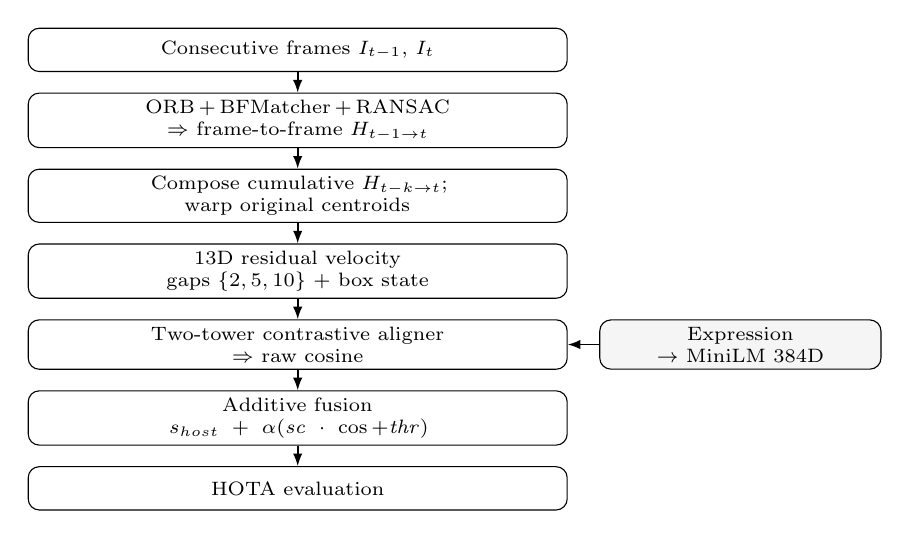
\begin{tikzpicture}[
  font=\scriptsize,
  node distance=2.6mm,
  box/.style={draw, rounded corners, align=center, inner sep=2.5pt,
              text width=0.55\linewidth, minimum height=5.5mm},
  sbox/.style={draw, rounded corners, align=center, inner sep=2.5pt, fill=black!4,
               text width=0.28\linewidth, minimum height=5.5mm},
  ar/.style={-{Latex[length=1.6mm]}, semithick}
]
\node[box] (frames) {Consecutive frames $I_{t-1},\,I_t$};
\node[box, below=of frames] (orb) {ORB\,+\,BFMatcher\,+\,RANSAC\\ $\Rightarrow$ frame-to-frame $H_{t-1\to t}$};
\node[box, below=of orb] (cum) {Compose cumulative $H_{t-k\to t}$;\\ warp original centroids};
\node[box, below=of cum] (desc) {13D residual velocity\\ gaps $\{2,5,10\}$ + box state};
\node[box, below=of desc] (align) {Two-tower contrastive aligner\\ $\Rightarrow$ raw cosine};
\node[box, below=of align] (fuse) {Additive fusion\\ $s_{\text{host}}+\alpha(\mathit{sc}\cdot\cos+\mathit{thr})$};
\node[box, below=of fuse] (hota) {HOTA evaluation};
\node[sbox, right=4mm of align] (text) {Expression\\ $\to$ MiniLM 384D};
\draw[ar] (frames)--(orb);
\draw[ar] (orb)--(cum);
\draw[ar] (cum)--(desc);
\draw[ar] (desc)--(align);
\draw[ar] (align)--(fuse);
\draw[ar] (fuse)--(hota);
\draw[ar] (text)--(align);
\end{tikzpicture}
\caption{GMC-Link pipeline. Consecutive frames feed an ORB homography estimate; transforms compose into a cumulative homography that yields a 13D residual-velocity descriptor; a two-tower encoder aligns the descriptor with the referring expression; the alignment score corrects the host logit through additive fusion, and the result is scored by HOTA.}
\label{fig:pipeline}
\end{figure}

\subsection{Ego-motion compensation}
\label{sec:ego}

The first stage recovers the camera transform between consecutive frames so that object displacement can later be separated from camera displacement. We detect ORB keypoints~\cite{orb} in both frames and match descriptors with a brute-force Hamming matcher, retaining a correspondence only when it passes Lowe's ratio test at $0.7$. Background dominates the matched set: we seed a foreground mask from the host's boxes in the previous frame and suppress keypoints inside them, so the surviving matches lie on static scene structure rather than on the moving objects themselves. RANSAC~\cite{ransac} then fits a $3\times3$ homography $H_{t-1\to t}$ to the masked correspondences, rejecting parallax outliers, and we record the median inlier reprojection error as a per-frame background residual. When too few inliers survive, the stage falls back to identity, so a frame with weak texture degrades to ``no compensation'' rather than to a corrupted estimate.

A single homography is exact only for planar or pure-rotation scenes. Driving footage is planar-dominated, which is why ORB with RANSAC outperformed dense optical flow on this data: the explicit outlier rejection discards the residual parallax that a flow field would smear into the estimate. Reasoning over a window of frames requires composing these transforms. Rather than warp coordinates iteratively, which accumulates interpolation error, we store the original never-warped object centroids and compose a single cumulative homography spanning $k$ frames,
\begin{equation}
H_{t-k\to t} = H_{t-1\to t}\, H_{t-2\to t-1} \cdots H_{t-k\to t-k+1},
\label{eq:cumulative}
\end{equation}
applying it once to map a past centroid into the current frame. One warp per query is numerically more stable than $k$ chained warps.

\subsection{Multi-scale residual velocity}
\label{sec:residual}

Compensated geometry lets us isolate true object motion. For a temporal gap $g$, the raw object velocity is the displacement of its centroid; the ego velocity is the displacement that the camera alone would induce, obtained by warping the past centroid through Eq.~\ref{eq:cumulative}. The residual velocity is their difference,
\begin{equation}
v^{\mathrm{res}}_{g} = v^{\mathrm{raw}}_{g} - v^{\mathrm{ego}}_{g},
\label{eq:residual}
\end{equation}
which is the motion a stationary camera would have observed. A parked car has near-zero residual velocity even while its pixels sweep across the frame, which is exactly the case that camera-naive hosts misread. We normalise each residual by image dimensions, $v_{\mathrm{norm}} = (v_{\mathrm{pix}}/d_{\mathrm{img}})\times 100$, so the representation is resolution-invariant and lands near unit magnitude.

We compute Eq.~\ref{eq:residual} at three frame gaps, $\{2,5,10\}$, to capture short, mid, and long-range motion in one descriptor. Concatenating these residuals with bounding-box state yields a 13-dimensional motion vector, $[\,\mathit{dx}_s,\ \mathit{dy}_s,\ \mathit{dx}_m,\ \mathit{dy}_m,\ \mathit{dx}_l,\ \mathit{dy}_l,\ \Delta w,\ \Delta h,\ c_x,\ c_y,\ w,\ h,\ \mathit{snr}\,]$, where the six leading entries are residual $(\mathit{dx},\mathit{dy})$ velocity pairs at gaps $2$, $5$, and $10$ rather than all-$x$ followed by all-$y$. The multi-scale design separates short jitter from sustained translation that a single gap conflates. A gap of $2$ resolves frame-to-frame jitter that a gap of $10$ averages away, while the gap of $10$ accumulates a slow drift that is buried in the noise of a single short step, so the three scales are complementary rather than redundant. The final entry, $\mathit{snr}$, is a signal-to-noise ratio: the mid-scale residual object speed divided by a background noise floor built from the buffer of RANSAC inlier residuals from Stage~1. It reports how trustworthy the compensation was on that frame; it leaves mean separation unchanged but reduces prediction variance by flagging frames where the homography was poorly constrained.

\subsection{Motion-language alignment}
\label{sec:align}

A lean two-tower encoder maps the 13D motion vector and the expression into a shared space. Each modality passes through a Linear adapter (motion $13\!\to\!256$, language $384\!\to\!256$, the latter from an all-MiniLM-L6-v2 SentenceTransformer~\cite{sbert}) into a shared MLP ($256\!\to\!512\!\to\!512\!\to\!256$) followed by layer normalisation and $\ell_2$ normalisation. We train it with a symmetric InfoNCE objective~\cite{infonce} at temperature $0.07$ and mask false negatives that arise when distinct samples share an expression. At inference we read the raw cosine similarity directly, with no sigmoid and no temporal smoothing, so the fusion stage receives an uncalibrated alignment score. This aligner is a standard contrastive component; its ceiling is representation-bound, and the design budget is spent on compensation and fusion rather than on the tower.

\subsection{Decision-level additive fusion}
\label{sec:fusion}

The alignment score corrects the host logit at the decision level. We inject it additively per host and per axis,
\begin{equation}
s_{\mathrm{final}} = s_{\mathrm{model}} + \alpha\,\bigl(\mathit{sc}\cdot\cos + \mathit{thr}\bigr),
\label{eq:fusion}
\end{equation}
where $\cos$ is the raw motion-language cosine, $\mathit{sc}$ rescales it onto the host's logit range, $\mathit{thr}$ shifts the operating point, and $\alpha$ sets the overall weight. Feature-level injection of motion into the visual encoder was catastrophic ($-21.7\%$ F1), which motivates keeping the correction at the decision layer where it cannot distort the host's appearance representation.

A keyword router classifies each expression as a motion query or an appearance query and selects the axis-specific recipe. The two axes differ sharply in their scale calibration: appearance expressions such as ``black cars'' carry no motion content, so the GMC score is noise on that axis and is damped by an $\mathit{sc}_{\mathrm{appear}}$ that is roughly seven to eleven times smaller than $\mathit{sc}_{\mathrm{motion}}$. The recipes also absorb the host logit scale, which differs by an order of magnitude between iKUN~\cite{ikun} (logits near $[0,1]$) and the FlexHook~\cite{flexhook} variants (logits near $[-10,10]$). Table~\ref{tab:recipe} lists the locked per-host coefficients; the same module attaches to any TransRMOT-lineage~\cite{transrmot} host through this calibration alone.

\begin{table}[t]
\centering
\caption{Locked per-host fusion coefficients for Eq.~\ref{eq:fusion}, by host and axis. Appearance scale is damped relative to motion scale because the motion signal is uninformative on appearance expressions.}
\label{tab:recipe}
\small
\begin{tabular}{llccc}
\toprule
Host & Axis & $\alpha$ & $\mathit{sc}$ & $\mathit{thr}$ \\
\midrule
\multirow{2}{*}{iKUN}        & motion     & 1.00 & 0.90 & $+0.17$ \\
                             & appearance & 1.00 & 0.30 & $+0.10$ \\
\midrule
\multirow{2}{*}{FlexHook-V1} & motion     & 0.65 & 10.0 & $+3.0$  \\
                             & appearance & 1.00 & 3.50 & $+0.9$  \\
\midrule
\multirow{2}{*}{FlexHook-V2} & motion     & 0.40 & 10.0 & $+1.3$  \\
                             & appearance & 1.00 & 3.50 & $+1.2$  \\
\bottomrule
\end{tabular}
\end{table}

These coefficients are scalars, not a learned head. We tried to derive them automatically by matching the standard deviations of the two score streams, and we tried replacing them with a learned fusion network; both underperformed the hand-set values, so the calibration stays a small fixed table that a new host can fit in a single pass without retraining its tracker.

\section{Experiments}
\label{sec:exp}

\subsection{Setup}
\label{sec:setup}

We evaluate on Refer-KITTI, the standard motion-aware RMOT benchmark, in two splits: Refer-KITTI V1~\cite{transrmot} (3-sequence pooled test) and its expanded relabeling Refer-KITTI V2~\cite{temprmot} (4-sequence pooled test). All scores are HOTA~\cite{hota} computed with TrackEval. Frame numbering must agree between the ground-truth template and the tracker output. We use the paper-canonical convention aligned with the NeuralSORT detections, under which the public iKUN~\cite{ikun} pipeline reproduces at $44.564$ pooled HOTA. The alternative regeneration is off by one frame and drops HOTA by roughly six points, so we do not use it. Every result with our module is reported as a mean over $n{=}3$ independent training seeds with its standard deviation. For each host we report two references: the unmodified host (\emph{native}) and the host fused with raw-cosine GMC scores under a simple, uncalibrated additive rule (\emph{+GMC simple}), which separates the value of the per-host recipe from the value of any GMC signal at all.

The test splits are heavily skewed toward appearance. V1 holds $158$ expressions over $1010$ frames, of which $75.3\%$ are appearance queries, $7.6\%$ are static-motion queries, and only $17.1\%$ ($27$ expressions) refer to a moving object; V2 holds $862$ expressions over $1469$ frames with a similar $74.1\,/\,11.7\,/\,14.2$ split. The motion class our module targets is therefore a roughly one-in-six minority of the test set. This shapes how the numbers should be read. Pooled HOTA averages over all expressions, so a large gain confined to the motion minority is diluted into a small pooled movement, and the pooled tenths understate the effect on the class the method is designed to fix. We treat per-class motion HOTA as the primary metric and report pooled HOTA alongside it.

\subsection{Main results}
\label{sec:main}

Table~\ref{tab:main} reports pooled HOTA for the three hosts, native and with the shipped module. On iKUN~\cite{ikun} the module reaches $44.634 \pm 0.066$, statistically indistinguishable from the host's own published $44.564$: it matches the pooled score rather than beating it. The motion-class breakdown explains where the effort goes. iKUN reads motion most weakly of the three hosts, and the module's per-class pooled gains land squarely on that deficit, with the largest single per-class delta of $+9.22$ on the iKUN moving class (Table~\ref{tab:deficit}). Across the nine host-by-class per-class pooled deltas (three hosts $\times$ motion/static/appearance), all nine are positive under $n{=}3$ evaluation. The pooled parity on iKUN is exactly the dilution effect: a large motion-class recovery spread over a $75\%$ appearance majority nets to no pooled movement. FlexHook-V2~\cite{flexhook} shows the clean pooled improvement, reaching $42.807 \pm 0.038$ against the host's published $42.526$, a gain of $+0.281$ that survives the appearance dilution. FlexHook-V1 improves over the \emph{+GMC simple} anchor ($53.121 \to 53.526$) but retains a residual gap to its own published number.\footnote{The FlexHook-V1 published pooled HOTA is $53.824$, which neither the shipped module ($53.526$, $\Delta=-0.298$) nor any tested configuration beats; the gap is structural rather than a tuning artifact, and we treat the V1 paper comparison as out of scope under the FlexHook split convention while reporting the gain against the \emph{+GMC simple} anchor.}

\begin{table}[t]
\centering
\caption{Pooled HOTA on Refer-KITTI test, native host versus the shipped GMC module ($n{=}3$, mean$\pm$std). $\Delta$ is against each host's published pooled HOTA. iKUN \emph{matches} its paper score while lifting the motion class (Table~\ref{tab:deficit}); FlexHook-V2 is the clean pooled improvement. The \emph{+GMC simple} control column is the simple-recipe anchor ($\alpha{=}1$, $sc{=}1$, $thr{=}0$, raw cosine, sw aligner, $n{=}3$).}
\label{tab:main}
\small
\setlength{\tabcolsep}{4pt}
\begin{tabular}{lcccc}
\toprule
Host & Native & +GMC simple & +GMC (ship) & $\Delta$ paper \\
\midrule
iKUN~\cite{ikun} (V1)        & 44.564 & 44.272 & $44.634 \pm 0.066$ & $+0.070$ \\
FlexHook-V1~\cite{flexhook}  & 53.824 & 53.121 & $53.526 \pm 0.087$ & $-0.298$\textsuperscript{$\dagger$} \\
FlexHook-V2~\cite{flexhook}  & 42.526 & 42.532 & $42.807 \pm 0.038$ & $+0.281$ \\
\bottomrule
\end{tabular}
\\[2pt]
{\footnotesize \textsuperscript{$\dagger$}FlexHook-V1 paper gap is structural (no tested configuration beats $53.824$); $\Delta$ vs \emph{+GMC simple} anchor $= +0.405$.}
\end{table}

\subsection{The motion deficit}
\label{sec:deficit}

The size of the gain is not uniform across hosts; it tracks how much motion ability each host lacks to begin with. Table~\ref{tab:deficit} pairs each host's native moving-class HOTA with the moving-class gain the module adds. iKUN starts at the lowest native moving-class ability and gains the most ($+9.22 \pm 0.88$); FlexHook-V1 starts higher and gains little ($+0.91 \pm 0.79$); FlexHook-V2 starts highest and gains almost nothing ($+0.43 \pm 0.17$), all over $n{=}3$ seeds. The relationship across the three hosts is monotone-inverse: a host with a larger motion deficit receives a larger motion-class correction. We do not state this as a proportional law; three hosts cannot support one. What it does support is a prediction, and the two FlexHook hosts are the predicted cross-host cases where a small deficit yields a small gain, consistent with the module supplying motion evidence only where the host fails to.

\begin{table}[t]
\centering
\caption{Motion deficit across hosts. Native moving-class HOTA versus the moving-class HOTA gain added by the module. The gain is monotone-inverse to native motion ability across the three hosts.}
\label{tab:deficit}
\small
\begin{tabular}{lcc}
\toprule
Host & Native MOVING & GMC MOVING gain ($n{=}3$) \\
\midrule
iKUN~\cite{ikun}             & 20.25 & $+9.22 \pm 0.88$ \\
FlexHook-V1~\cite{flexhook}  & 43.98 & $+0.91 \pm 0.79$ \\
FlexHook-V2~\cite{flexhook}  & 48.02 & $+0.43 \pm 0.17$ \\
\bottomrule
\end{tabular}
\end{table}

\subsection{Ablations}
\label{sec:ablation}

To locate where the recovery comes from, we strip the module one component at a time and read the moving-class HOTA, the metric the pooled score hides. Table~\ref{tab:ablation} reports the full module against three reductions: replacing residual velocity with raw, uncompensated velocity (\emph{-ego}); collapsing the three temporal gaps to one (\emph{-multiscale}); and removing the signal-to-noise feature (\emph{-snr}). The recovery is carried first by the module itself: aligning motion with language lifts the moving class from $20.25$ to $29.47$ ($+9.22$ over the native host). Among the engineered components, ego-compensation is the only one whose removal moves the metric beyond seed noise: feeding raw velocity, which carries the camera's motion intact, costs $-1.88$ and gives back roughly a fifth of the module's gain, confirming that compensation contributes over and above merely having a motion descriptor. Collapsing the temporal scales ($-0.56$) and removing snr ($+0.40$) both stay within seed noise, so neither is load-bearing on this metric; the multi-scale and snr designs earn their place as resolution and robustness choices rather than as measured moving-class gains.

\begin{table}[t]
\centering
\caption{Component ablation in moving-class HOTA (the metric pooled scores dilute), iKUN host, $n{=}3$ seeds (mean$\,\pm\,$std). Against the native host (20.25), the full module recovers $+9.22$; among the engineered components only ego-compensation moves the metric beyond seed noise ($-1.88$), while collapsing the temporal scales or removing snr stay within it.}
\label{tab:ablation}
\small
\begin{tabular}{lc}
\toprule
Variant & MOVING HOTA \\
\midrule
Native host (no module)           & 20.25 \\
Full module                       & \textbf{29.47 $\pm$ 0.88} \\
\;\;$-$ego (raw velocity)         & 27.59 $\pm$ 0.12 \\
\;\;$-$multiscale (single gap)    & 28.91 $\pm$ 1.17 \\
\;\;$-$snr                        & 29.87 $\pm$ 0.75 \\
\bottomrule
\end{tabular}
\end{table}

The injection site is as consequential as the signal. Injecting motion features into the visual encoder, rather than fusing at the decision level, regresses the host by $-21.7\%$ F1, which is why the module corrects the logit after the host has scored appearance rather than reshaping the host's representation.

\begin{figure}[t]
\centering
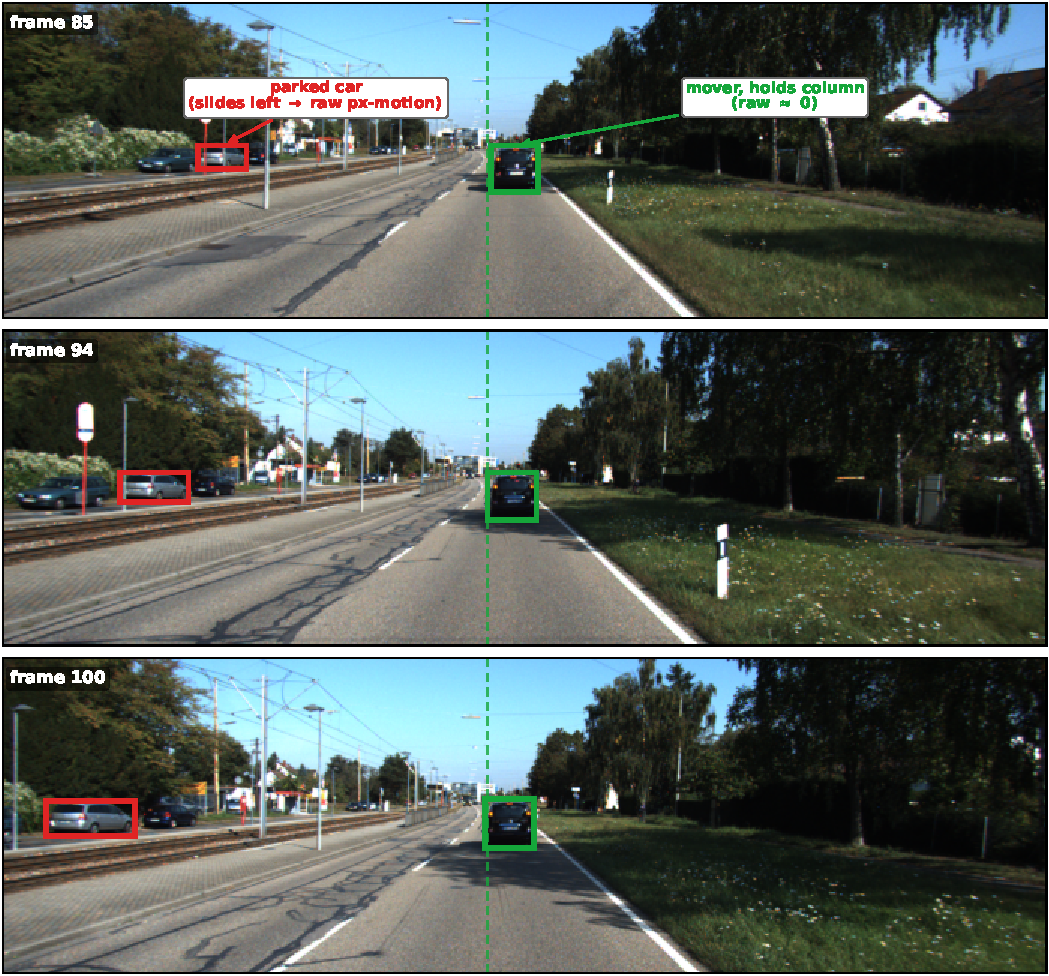
\includegraphics[width=\linewidth]{figures/qualitative.pdf}
\caption{Real recovery under camera ego-motion on the expression ``moving cars'' (Refer-KITTI, sequence 0005, frames 85/94/100 of a forward-driving clip; ground truth: the green car moves, the red car is parked). The dashed green line marks the mover's image column. \textbf{Red:} a parked car whose image-plane centroid slides left across the strip as the camera passes it (center-$x$ $261\!\to\!104$\,px, ${\approx}10$\,px/frame), drifting off the dashed line; the camera-naive host reads this raw displacement and scores it ``moving'' (a false positive), yet its ego-compensated residual is near zero and the module restores it to static. \textbf{Green:} a car keeping pace with traffic holds that column (center-$x$ ${\approx}605$, ${<}1$\,px/frame), so the host misses it (a false negative); the residual is nonzero --- it does not move like the static background --- and the module recovers it as moving. Both errors flip from the same host logit through the additive correction.}
\label{fig:qual}
\end{figure}

An appearance re-ranker orthogonal to the motion module stacks on iKUN to $45.612$ pooled HOTA ($+1.032$), the first iKUN pooled result above $45.5$; it targets the appearance majority rather than the motion class and is detailed in the supplement. The full pipeline runs at roughly $57$--$61$ FPS on CPU, about $6$--$8\times$ the $10$~fps capture rate of the benchmark, so the compensation adds no practical inference burden.

\section{Conclusion and Limitations}
\label{sec:conclusion}
A plug-in decision-level module that compensates camera ego-motion recovers the motion-class referring expressions that camera-naive hosts systematically miss. The recovered signal grows as the host's own ability to read object motion shrinks: across the three hosts studied, the gain is monotone-inverse to native motion ability, largest where the host is most motion-blind and small where the host already reads motion well. The module delivers this at a fixed tracker, retraining neither the host nor swapping the detector, and adds only a small per-host scalar calibration. On iKUN~\cite{ikun} it matches the published pooled HOTA while lifting the motion class the pooled number hides; on FlexHook-V2~\cite{flexhook} it improves the pooled score outright.

We frame the open issues as bounded failure modes, each with the mechanism that bounds it. The compensation rests on a single homography per frame, which is exact only for planar or pure-rotation scenes. Driving is planar-dominated, and the parallax that survives the ORB-and-RANSAC fit is discarded as outliers and further absorbed by an aligner trained on jittered, imperfect motion, so strong parallax is bounded at two stages rather than left to corrupt the descriptor. The foreground mask is seeded from the host's own boxes, so a badly wrong detection can leak object features into the ego estimate. RANSAC outlier rejection and an identity-homography fallback bound that leakage, so compensation degrades gracefully with detection quality rather than failing catastrophically. The gains hold at a fixed tracker and are orthogonal to detector quality rather than dependent on it; reaching the top of the leaderboard requires a stronger tracker than the public detections expose, which is out of scope. The alignment ceiling is set by what a 2D kinematic descriptor can encode, not by the fusion stage. Finally, hosts with native temporal memory, such as TempRMOT~\cite{temprmot}, fall outside our target: their recurrent state already aggregates trajectory history, making an external motion module redundant rather than complementary.

The open lever is a stronger motion representation. Because the alignment ceiling sits in the descriptor rather than in the fusion stage that consumes it, future work points at richer motion features that encode the trajectory geometry a 2D kinematic vector flattens. The TransRMOT~\cite{transrmot} lineage of camera-naive hosts is where that headroom lies.

\bibliographystyle{ACM-Reference-Format}
\bibliography{refs}

\end{document}
